\begin{minipage}{0.75\linewidth}
\begin{figure}[h]
    \centering
    \begin{adjustbox}{max width=1.0\linewidth, keepaspectratio}
        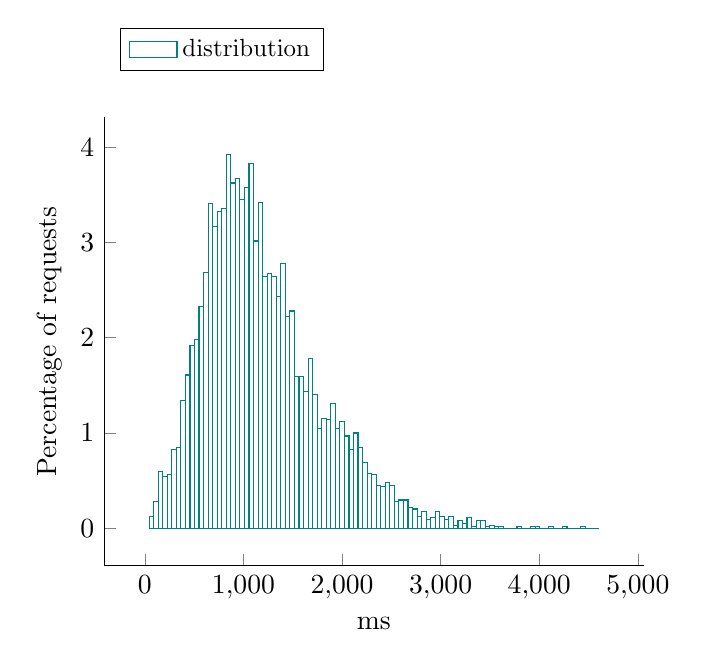
\begin{tikzpicture}
            \begin{axis}[ylabel = Percentage of requests, 
xlabel = ms, 
legend style = {nodes={scale=0.9, transform shape}, at={(0.03,1.2)}, anchor=north west, draw=black, fill=white, align=left, legend columns=3},
area style, mark size = 0pt,
 cycle list name = exotic,
  axis lines* = left]
		\addplot +[ybar interval] coordinates {
			 (43, 0.125)
			 (89.07, 0.28125)
			 (135.14, 0.59375)
			 (181.21, 0.546875)
			 (227.28, 0.5625)
			 (273.35, 0.828125)
			 (319.42, 0.84375)
			 (365.49, 1.34375)
			 (411.56, 1.60938)
			 (457.63, 1.92188)
			 (503.7, 1.98438)
			 (549.77, 2.32812)
			 (595.84, 2.6875)
			 (641.91, 3.40625)
			 (687.98, 3.17187)
			 (734.05, 3.32812)
			 (780.12, 3.35938)
			 (826.19, 3.92187)
			 (872.26, 3.625)
			 (918.33, 3.67188)
			 (964.4, 3.45312)
			 (1010.47, 3.57812)
			 (1056.54, 3.82813)
			 (1102.61, 3.01562)
			 (1148.68, 3.42188)
			 (1194.75, 2.64062)
			 (1240.82, 2.67188)
			 (1286.89, 2.64062)
			 (1332.96, 2.4375)
			 (1379.03, 2.78125)
			 (1425.1, 2.21875)
			 (1471.17, 2.28125)
			 (1517.24, 1.59375)
			 (1563.31, 1.59375)
			 (1609.38, 1.4375)
			 (1655.45, 1.78125)
			 (1701.52, 1.40625)
			 (1747.59, 1.04688)
			 (1793.66, 1.15625)
			 (1839.73, 1.14062)
			 (1885.8, 1.3125)
			 (1931.87, 1.04688)
			 (1977.94, 1.125)
			 (2024.01, 0.96875)
			 (2070.08, 0.828125)
			 (2116.15, 1)
			 (2162.22, 0.84375)
			 (2208.29, 0.6875)
			 (2254.36, 0.578125)
			 (2300.43, 0.5625)
			 (2346.5, 0.453125)
			 (2392.57, 0.4375)
			 (2438.64, 0.484375)
			 (2484.71, 0.453125)
			 (2530.78, 0.28125)
			 (2576.85, 0.296875)
			 (2622.92, 0.296875)
			 (2668.99, 0.21875)
			 (2715.06, 0.203125)
			 (2761.13, 0.125)
			 (2807.2, 0.171875)
			 (2853.27, 0.09375)
			 (2899.34, 0.109375)
			 (2945.41, 0.171875)
			 (2991.48, 0.125)
			 (3037.55, 0.09375)
			 (3083.62, 0.125)
			 (3129.69, 0.03125)
			 (3175.76, 0.078125)
			 (3221.83, 0.046875)
			 (3267.9, 0.109375)
			 (3313.97, 0.015625)
			 (3360.04, 0.078125)
			 (3406.11, 0.078125)
			 (3452.18, 0.015625)
			 (3498.25, 0.03125)
			 (3544.32, 0.015625)
			 (3590.39, 0.015625)
			 (3636.46, 0)
			 (3682.53, 0)
			 (3728.6, 0)
			 (3774.67, 0.015625)
			 (3820.74, 0)
			 (3866.81, 0)
			 (3912.88, 0.015625)
			 (3958.95, 0.015625)
			 (4005.02, 0)
			 (4051.09, 0)
			 (4097.16, 0.015625)
			 (4143.23, 0)
			 (4189.3, 0)
			 (4235.37, 0.015625)
			 (4281.44, 0)
			 (4327.51, 0)
			 (4373.58, 0)
			 (4419.65, 0.015625)
			 (4465.72, 0)
			 (4511.79, 0)
			 (4557.86, 0)
			 (4603.93, 0.015625)
		};
\addlegendentry{distribution};
           \end{axis}
      \end{tikzpicture}
  \end{adjustbox}
  \caption{Response time distribution - req = ReadTimeline-3}
\end{figure}
\end{minipage}\hfill\begin{minipage}{0.18\linewidth}
\begin{table}[h]
\begin{tabular}{|cc|}
\hline
\textbf{} & \textbf{ms}\\ \hline
 \Xhline{0.005\arrayrulewidth}
min & 43\\
 \Xhline{0.005\arrayrulewidth}
max & 4650\\
 \Xhline{0.005\arrayrulewidth}
mean & 1200\\
 \Xhline{0.005\arrayrulewidth}
std & 599\\
\hline
\hline
 \Xhline{0.005\arrayrulewidth}
25th & 773\\
 \Xhline{0.005\arrayrulewidth}
50th & 1090\\
 \Xhline{0.005\arrayrulewidth}
75th & 1515\\
 \Xhline{0.005\arrayrulewidth}
80th & 1664\\
 \Xhline{0.005\arrayrulewidth}
85th & 1834\\
 \Xhline{0.005\arrayrulewidth}
90th & 2035\\
 \Xhline{0.005\arrayrulewidth}
95th & 2331\\
 \Xhline{0.005\arrayrulewidth}
99th & 2989\\
\hline
\end{tabular}
\caption{Response time}
\end{table}
\end{minipage}\hfill